\section{Code and Carrier}

The measurements in the global navigation satellite system are mainly characterized by the measurement of time. The satellites use atomic clocks due to the sensitivity in the calculation of the position given the very high speed with respect to which they orbit, which also produces certain relativistic effects.\\

\begin{figure}[H]
        \centering
        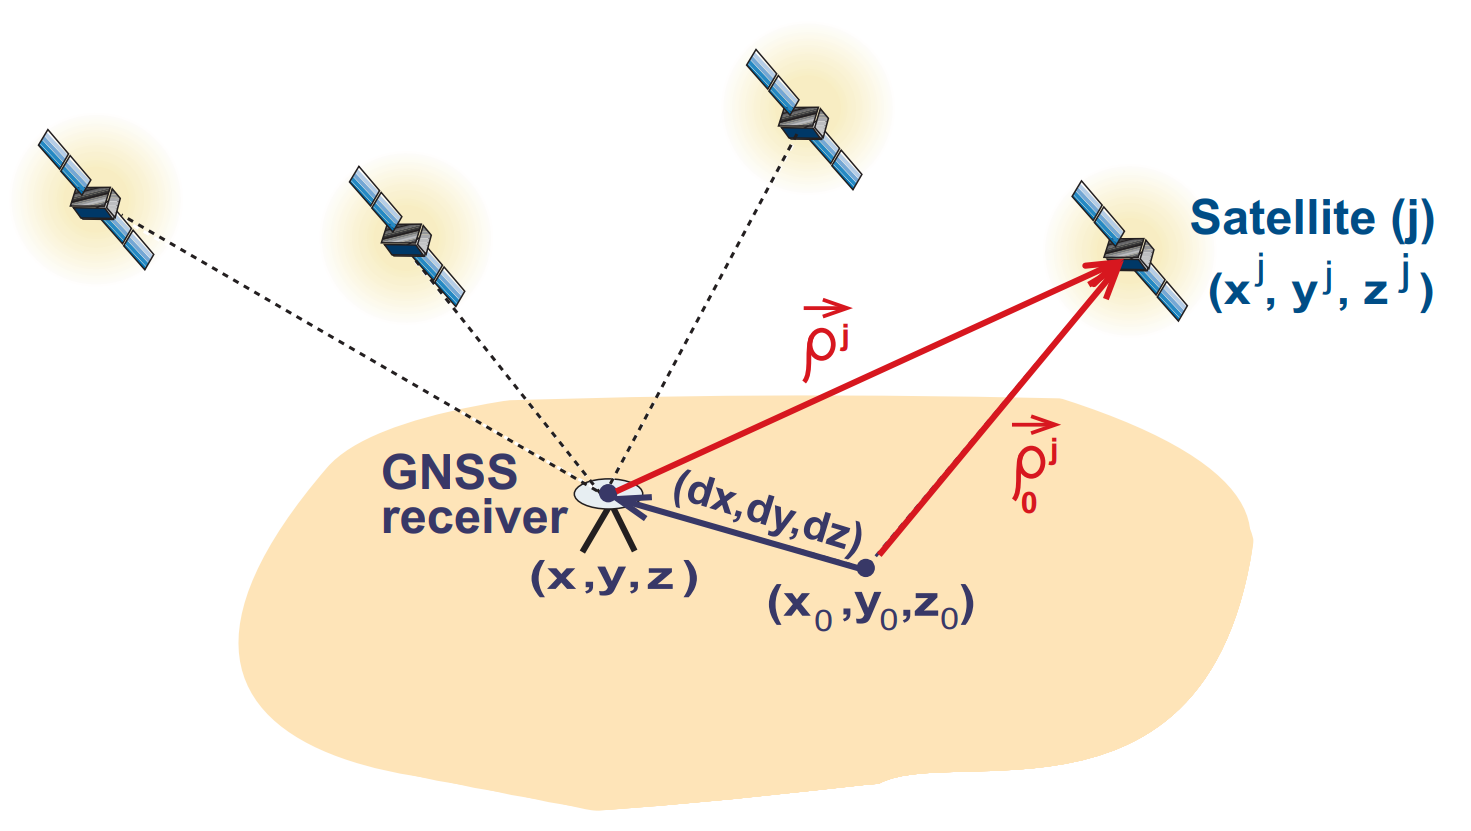
\includegraphics[scale=0.27]{sources/Figures/GNSS_Scheme.png}
        \caption{GNSS Schematic}
        \label{fig:radio magnetic}
\end{figure}


Satellites transmit their positions through "Code" and "Carrier"  \vartext{P_{1}-P_{2}} and \vartext{L_{1}-L_{2}} signals respectively, which contain orbital and time information (\vartext{L1 = 1575.42 MHz} and \vartext{L_{2} = 1227.6 MHz}). The receiver calculates its geographical location by comparing the transmission and reception times of signals received from different satellites. However, the codes must be designed to avoid errors caused by factors such as SNR \fnote{SNR} reduction due to the ionosphere and other electronic losses.

\section{Geometric Range}

To mitigate these errors, filters are employed like the Kalman filter. The Pseudorange-Based Algorithm is used to compute the position, which involves calculating the Euclidean distance from the receiver to each satellite while accounting for noise and time offsets. 

The geometric range $\rho_{rcv}^{sat}$ is computed using the Euclidean distance (see references \citeblue{subirana2013gnss} and \citeblue{HernandezEtAl_GPSDataProcessing}).

\begin{equation}\label{Geometric Range}
    \rho_{rcv}^{sat} = \mid\mid r^{sat}-r_{rcv} \mid\mid = 
\sqrt{\left(x^{sat}-x_{rcv}\right)^{2}+\left(y^{sat}-y_{rcv}\right)^{2}+\left(z^{sat}-z_{rcv}\right)^{2}}
\end{equation}

The measurement \vartext{R = c\Delta T} is the pseodurange mentioned before. This distance is called this way because it is not a real Range distance, but the ones generated by losses due to noise due to atmospheric, electronic and multipath factors are added to the geometric range.

\section{Pseudorange}
For a reference time scale $T$ and using the code $P$ for the frequency signal $f$, the pseudorange for the satellite and receiver is as follows:

\begin{equation}\label{Simple Pseudorange}
    R_{P_{f}} = c\left[t_{rcv}\left(T_{2}\right)-t^{sat} \left(T_{}\right)\right]
\end{equation}

where: $c$ is the speed of light in vacuum, $t_{rcv}\left(T_{2}\right)$ is the time of signal reception, and $t^{sat} \left(T_{}\right)$ the of signal transmission. The time of reception is measured by the receiver clock and the transmission time is measured by the satellite clock.


Then, the pseudorange \vartext{R_{P_{f}}} obtained by the receiver that includes the \vartext{\rho} geometric range between the receiver and the satellite including clock offsets including relativistic effects \vartext{dt_{rcv}} and \vartext{dt^{sat}} and the other terms due to the signal propagation, like ionosphere frequency-dependent delay \vartext{\alpha STEC}\fnote{STEC}, troposphere delay \vartext{Tr}, instrumental frequency and code-dependent delays \vartext{K_{P_{f,rcv}}} and \vartext{K_{P_{f}}^{sat}, receiver \ noise \ \epsilon _{P_{f}}} and multipath effects \vartext{M_{P_{f}}}.



\begin{equation}\label{Pseudorange}
    R_{P_{f}} = \rho + c \left( dt_{rcv} - dt^{sat} \right) + Tr + \alpha STEC + K_{P_{f,rcv}} - K_{P_{f}}^{sat} + M_{P_{f}} + \epsilon _{P_{f}}
\end{equation}


where, \vartext{\alpha_{f} = \frac{40.3}{f^2}10^{16} \ m_{(signal \ delay \ at \ frequency \  f)}/TECU} and \vartext{1 \ TECU = 10^{16}e^{-}/m^{2}}\footnote{\ac{TECU}}.\\


\begin{figure}[H]
        \centering
        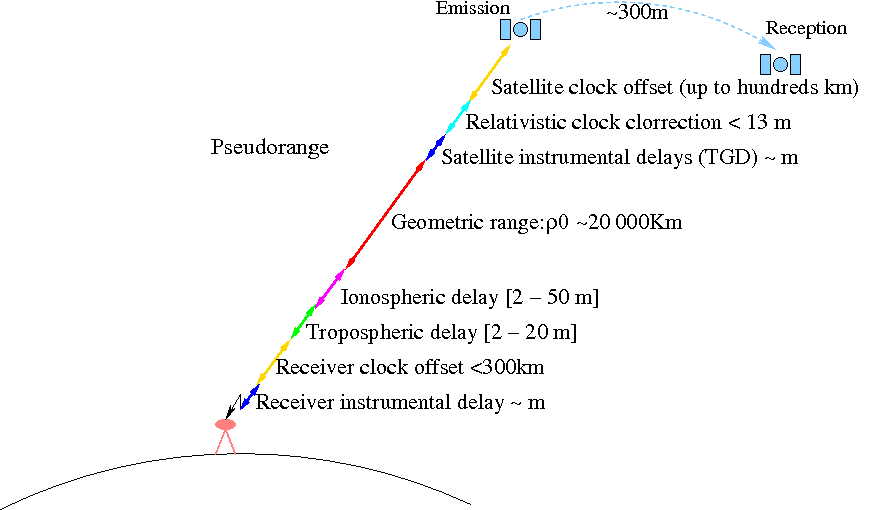
\includegraphics[scale=0.4]{sources/Figures/ranges.png}
        \caption{Pseudorange measurement content \citeblue{GNSSmeasurement}}
        \label{fig:Pseudorange measurement content}
\end{figure}


This is a simple reminder of the different equations that are used to calculate the distances of a receiver with respect to each one of the satellites, being necessary as a minimum of at least 4 satellites (for the precise positioning pointing 5 satellites are needed)so that the receiver can compute the three Cartesian components of the space and time. Otherwise, with more satellites, the precision increases but also the noise of the signal due to the superposition of radio waves.

For a \ac{PPP} a linear model is used following the same procedure as with the \ac{SPP}.

